\subsection{Motivated Beliefs vs. Informed Beliefs: The Epistemic Foundation of Awareness}
\label{subsec:11-3-motivated-beliefs}

%%%%%%%%%%%%%%%%%%%%%%%%%%%%%%%%%%%%%%%%%%%%%%%%%%%%%%%%%%%%%%%%%%%%%%%%%%%%%%%
% SECTION 11.03: Motivated vs. Informed Beliefs
% Position: After Definition (11.01) and Moment of Truth (11.02)
% Before: System Levels, Transformation Equation
% Rationale: Beliefs are CONSTITUTIVE for Awareness, not an add-on
% Key references: Bénabou (2015), Bénabou & Tirole (2011, 2016)
%%%%%%%%%%%%%%%%%%%%%%%%%%%%%%%%%%%%%%%%%%%%%%%%%%%%%%%%%%%%%%%%%%%%%%%%%%%%%%%

Section~\ref{subsec:awareness-definition} defined awareness as consciousness 
of utility effects at the Moment of Truth. But this raises a prior question: 
\emph{What determines which effects enter consciousness?} 

The answer involves \textbf{beliefs}---and beliefs themselves are not neutral 
information processors. This section establishes that the Awareness function 
$A$ is fundamentally shaped by whether beliefs are \emph{informed} (evidence-driven) 
or \emph{motivated} (desire-driven).

\begin{tcolorbox}[colback=red!5!white, colframe=red!75!black, title=Why This Section Comes Early]
Beliefs are not an extension of the Awareness framework---they are 
\textbf{constitutive} of it. One cannot specify $A$ without understanding 
how beliefs filter information before it reaches consciousness. The 
transformation equation (Section~\ref{subsec:11-6-transformation-equation}) 
presupposes this epistemic foundation.
\end{tcolorbox}

%------------------------------------------------------------------------------
\subsubsection{The Core Distinction}
\label{subsubsec:core-distinction}
%------------------------------------------------------------------------------

\begin{tcolorbox}[colback=blue!5!white, colframe=blue!75!black, title=Two Modes of Belief Formation]
\textbf{Informed Beliefs}: Evidence $\rightarrow$ Belief \\
Beliefs are updated according to Bayes' rule to maximize predictive accuracy.

\textbf{Motivated Beliefs}: Desire $\rightarrow$ Belief \\
Beliefs are shaped by what the agent \emph{wants} to believe, trading accuracy 
for psychological benefits.
\end{tcolorbox}

This distinction, developed systematically by Bénabou and Tirole across two 
decades of research, is foundational for the Awareness function.

\paragraph{The Bénabou Research Program.}
The economics of motivated beliefs emerged from sustained theoretical work:

\begin{table}[htbp]
\centering
\caption{Key Papers in the Economics of Motivated Beliefs}
\label{tab:benabou-papers}
\renewcommand{\arraystretch}{1.3}
\small
\begin{tabular}{@{}llp{5.5cm}@{}}
\toprule
\textbf{Year} & \textbf{Paper} & \textbf{Core Contribution} \\
\midrule
2002 & Self-Confidence (QJE) & Memory management for self-motivation \\
2004 & Willpower (JPE) & Personal rules as self-reputation \\
2006 & Just World (QJE) & Political ideology as motivated belief \\
2011 & Identity, Morals, Taboos (QJE) & Beliefs as assets with supply/demand \\
2013 & Groupthink (REStud) & Collective reality denial \\
2015 & Economics of Motivated Beliefs & Unified model (Laffont Lecture) \\
2016 & Mindful Economics (JEP) & Synthesis: beliefs as economic goods \\
\bottomrule
\end{tabular}
\end{table}

\paragraph{The Central Insight.}
Bénabou and Tirole (2016) propose treating beliefs ``as regular economic goods 
and assets---which people consume, invest in, reap returns from, and produce, 
using the informational inputs they receive or have access to.''

%------------------------------------------------------------------------------
\subsubsection{Formal Framework: The Belief Utility Model}
\label{subsubsec:formal-framework}
%------------------------------------------------------------------------------

Following Bénabou (2015), an agent's total utility from holding belief 
$\hat{\theta}$ about state $\theta$ is:

\begin{equation}
\label{eq:belief-utility}
V(\hat{\theta}) = \underbrace{U_{accuracy}(\hat{\theta}, \theta)}_{\text{Instrumental value}} + \underbrace{U_{psychological}(\hat{\theta})}_{\text{Consumption value}}
\end{equation}

\paragraph{Instrumental Value.}
Accurate beliefs enable better decisions:
\begin{equation}
U_{accuracy} = -c \cdot (\hat{\theta} - \theta)^2
\end{equation}
where $c > 0$ is the cost of prediction errors.

\paragraph{Psychological Value.}
Certain beliefs generate direct utility:
\begin{equation}
U_{psychological} = \alpha \cdot \hat{\theta}
\end{equation}
where $\alpha > 0$ captures the ``desirability'' of optimistic beliefs.

\paragraph{Optimal Motivated Belief.}
The agent chooses $\hat{\theta}$ to maximize total utility:
\begin{equation}
\hat{\theta}^* = \theta + \frac{\alpha}{2c}
\end{equation}

This yields a systematic \textbf{optimistic bias} proportional to:
\begin{itemize}
\item $\alpha$: How much the agent values positive beliefs
\item $1/c$: How little accuracy matters instrumentally
\end{itemize}

%------------------------------------------------------------------------------
\subsubsection{Three Sources of Belief-Based Utility}
\label{subsubsec:three-sources}
%------------------------------------------------------------------------------

Bénabou and Tirole (2016) identify three mechanisms generating demand for 
motivated beliefs:

\begin{table}[htbp]
\centering
\caption{Three Sources of Belief-Based Utility}
\label{tab:three-sources}
\renewcommand{\arraystretch}{1.4}
\begin{tabular}{@{}lp{4.2cm}p{4.8cm}@{}}
\toprule
\textbf{Source} & \textbf{Mechanism} & \textbf{EBF Link} \\
\midrule
\textbf{Anticipatory Utility} & 
Future-oriented emotions (hope, anxiety) depend on beliefs &
$U^{INU}_{G,2-4}$, $U^{INU}_{P,2-4}$ \\
\textbf{Ego/Self-Image Utility} & 
Self-esteem depends on beliefs about own abilities &
$U^{IDN}$ (Identity Utility) \\
\textbf{Functional Value} & 
Beliefs affect motivation, thus actual outcomes &
SYS 2 $\rightarrow$ Effort $\rightarrow$ Performance \\
\bottomrule
\end{tabular}
\end{table}

%------------------------------------------------------------------------------
\subsubsection{Supply Side: How Motivated Beliefs Are Produced}
\label{subsubsec:supply-side}
%------------------------------------------------------------------------------

If there is demand for motivated beliefs, there must be mechanisms to 
\emph{produce} them:

\begin{table}[htbp]
\centering
\caption{Mechanisms of Belief Production}
\label{tab:supply-mechanisms}
\renewcommand{\arraystretch}{1.3}
\begin{tabular}{@{}lp{5cm}@{}}
\toprule
\textbf{Mechanism} & \textbf{Description} \\
\midrule
Selective Memory & Forget negative signals, remember positive \\
Selective Attention & Focus on confirming evidence \\
Biased Interpretation & Interpret ambiguous evidence favorably \\
Information Avoidance & Choose not to receive threatening info \\
Self-Signaling & Infer values from own actions \\
\bottomrule
\end{tabular}
\end{table}

%------------------------------------------------------------------------------
\subsubsection{Integration into the Awareness Function}
\label{subsubsec:awareness-integration}
%------------------------------------------------------------------------------

This is the critical section: How do motivated beliefs affect $A$?

\paragraph{The Standard View (Incomplete).}
The naive specification treats awareness as a function of external factors only:
\begin{equation}
A_X = f(\text{Salience}, \text{Availability}, \text{Framing}, ...)
\end{equation}

This is incomplete because it ignores that \textbf{beliefs pre-filter what 
becomes salient, available, and how frames are processed}.

\paragraph{The Extended Awareness Function.}
We introduce the \textbf{Belief Filter} $B$:

\begin{equation}
\boxed{
A_X(t^*) = A^{base}_X(t^*) \times B_X(\hat{\theta}, signal, U_{IDN})
}
\label{eq:awareness-belief-filter}
\end{equation}

where:
\begin{itemize}
\item $A^{base}_X$ = Awareness from external factors (salience, etc.)
\item $B_X$ = Belief Filter (endogenous, motivated)
\item $\hat{\theta}$ = Current belief state
\item $signal$ = Incoming information
\item $U_{IDN}$ = Identity utility at stake
\end{itemize}

\paragraph{The Belief Filter Specification.}

\begin{equation}
B_X(\hat{\theta}, signal) = 
\begin{cases}
1 & \text{if } signal \text{ is belief-consistent} \\[8pt]
1 - \lambda \cdot \left| \dfrac{\partial U_{IDN}}{\partial \hat{\theta}} \right| & \text{if } signal \text{ is belief-inconsistent}
\end{cases}
\label{eq:belief-filter}
\end{equation}

where $\lambda \in [0,1]$ is the \textbf{motivation strength parameter}.

\paragraph{Interpretation.}
\begin{itemize}
\item When $\lambda = 0$: No motivated cognition; $B = 1$ always (rational benchmark)
\item When $\lambda = 1$: Full motivated cognition; threatening signals suppressed 
      proportionally to identity stakes
\item The term $\left| \frac{\partial U_{IDN}}{\partial \hat{\theta}} \right|$ 
      captures how much identity utility depends on the belief
\end{itemize}

%------------------------------------------------------------------------------
\subsubsection{The Complete Awareness Architecture}
\label{subsubsec:complete-architecture}
%------------------------------------------------------------------------------

Combining the Belief Filter with the base awareness function:

\begin{figure}[htbp]
\centering
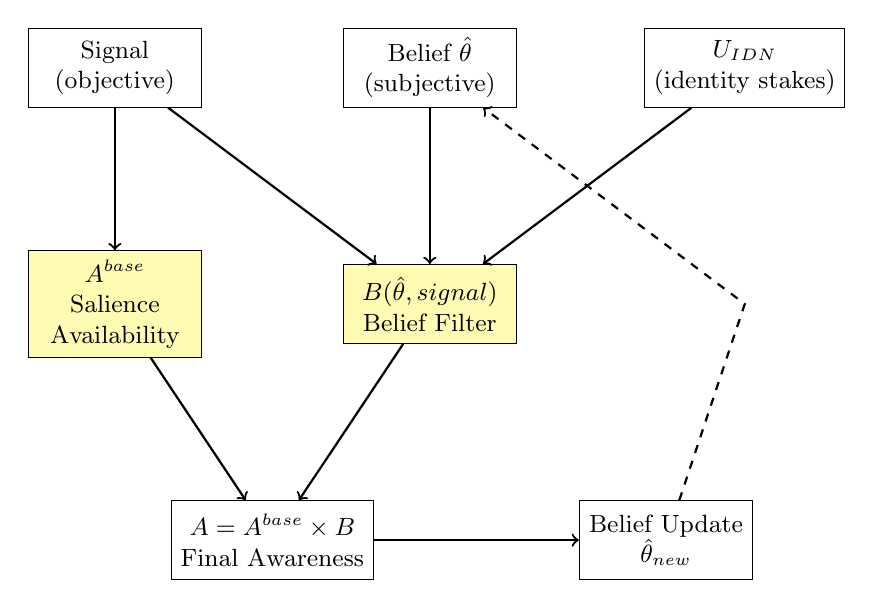
\begin{tikzpicture}[
    box/.style={rectangle, draw, minimum width=2.2cm, minimum height=1cm, align=center, font=\small},
    filter/.style={rectangle, draw, fill=yellow!30, minimum width=2.2cm, minimum height=1cm, align=center, font=\small},
    arrow/.style={->, thick},
    node distance=2.5cm
]

% Row 1: Inputs
\node[box] (signal) at (0,3) {Signal\\(objective)};
\node[box] (belief) at (4,3) {Belief $\hat{\theta}$\\(subjective)};
\node[box] (uidn) at (8,3) {$U_{IDN}$\\(identity stakes)};

% Row 2: Filters
\node[filter] (abase) at (0,0) {$A^{base}$\\Salience\\Availability};
\node[filter] (bfilter) at (4,0) {$B(\hat{\theta}, signal)$\\Belief Filter};

% Row 3: Output
\node[box] (afinal) at (2,-3) {$A = A^{base} \times B$\\Final Awareness};

% Arrows
\draw[arrow] (signal) -- (abase);
\draw[arrow] (signal) -- (bfilter);
\draw[arrow] (belief) -- (bfilter);
\draw[arrow] (uidn) -- (bfilter);
\draw[arrow] (abase) -- (afinal);
\draw[arrow] (bfilter) -- (afinal);

% Feedback loop
\node[box] (update) at (7,-3) {Belief Update\\$\hat{\theta}_{new}$};
\draw[arrow] (afinal) -- (update);
\draw[arrow, dashed] (update) -- (8,0) -- (belief);

\end{tikzpicture}
\caption{Complete Awareness Architecture with Belief Filter}
\label{fig:awareness-architecture}
\end{figure}

\paragraph{The Feedback Loop.}
The dashed arrow represents the critical feedback:
\begin{enumerate}
\item Beliefs filter what enters awareness
\item Filtered information updates beliefs
\item Updated beliefs filter future information
\item $\Rightarrow$ \textbf{Belief perseverance / confirmation bias}
\end{enumerate}

%------------------------------------------------------------------------------
\subsubsection{Formal Properties of the Belief Filter}
\label{subsubsec:formal-properties}
%------------------------------------------------------------------------------

\begin{tcolorbox}[colback=gray!5!white, colframe=gray!75!black, title=Property 1: Asymmetric Updating]
For belief-consistent signals: $B = 1$ (full awareness)\\
For belief-inconsistent signals: $B < 1$ (suppressed awareness)\\
$\Rightarrow$ Asymmetric information processing
\end{tcolorbox}

\begin{tcolorbox}[colback=gray!5!white, colframe=gray!75!black, title=Property 2: Stakes Dependence]
The suppression is proportional to identity stakes:
\begin{equation}
\frac{\partial B}{\partial |U_{IDN}|} < 0 \quad \text{for inconsistent signals}
\end{equation}
Higher identity stakes $\Rightarrow$ stronger filtering
\end{tcolorbox}

\begin{tcolorbox}[colback=gray!5!white, colframe=gray!75!black, title=Property 3: Domain Specificity]
$\lambda$ varies by domain:
\begin{itemize}
\item High $\lambda$: Politics, religion, moral self-image
\item Low $\lambda$: Technical domains, emotionally neutral topics
\end{itemize}
\end{tcolorbox}

%------------------------------------------------------------------------------
\subsubsection{EBF Integration: Beliefs Across Utility Categories}
\label{subsubsec:bcm-integration}
%------------------------------------------------------------------------------

The Belief Filter operates differently across utility categories:

\begin{table}[htbp]
\centering
\caption{Belief Filter by Utility Category}
\label{tab:beliefs-by-category}
\renewcommand{\arraystretch}{1.4}
\begin{tabular}{@{}llll@{}}
\toprule
\textbf{Category} & \textbf{Belief Content} & \textbf{$\lambda$ (typical)} & \textbf{Implication} \\
\midrule
\textbf{INU} & Abilities, outcomes & Low--Medium & Feedback can correct \\
\textbf{KNU} & Group efficacy & Medium & Social reinforcement \\
\textbf{IDN} & Values, moral character & \textbf{High} & Strong filtering \\
\bottomrule
\end{tabular}
\end{table}

\paragraph{Critical Insight.}
The Belief Filter is strongest in the \textbf{IDN} category because:
\begin{enumerate}
\item Identity beliefs are harder to falsify empirically
\item They are more emotionally charged
\item The self-image stakes ($U_{IDN}$) are highest
\end{enumerate}

This explains the empirical pattern that \textbf{identity-relevant information 
is processed most asymmetrically}.

%------------------------------------------------------------------------------
\subsubsection{Informed Beliefs: The Rational Benchmark}
\label{subsubsec:informed-beliefs}
%------------------------------------------------------------------------------

When $\lambda = 0$, the Belief Filter disappears and we recover Bayesian updating:

\begin{equation}
\hat{\theta}_{t+1} = \frac{Pr(signal | \theta = H) \cdot \hat{\theta}_t}{Pr(signal | \theta = H) \cdot \hat{\theta}_t + Pr(signal | \theta = L) \cdot (1-\hat{\theta}_t)}
\end{equation}

\paragraph{Properties of Informed Beliefs.}
\begin{enumerate}
\item \textbf{Symmetric updating}: Good and bad news weighted equally
\item \textbf{Convergence}: Beliefs converge to truth with evidence
\item \textbf{Information seeking}: More information is always valuable
\end{enumerate}

\paragraph{When Are Beliefs Informed?}
\begin{itemize}
\item Stakes for accuracy are high ($c$ large)
\item Psychological stakes are low ($\alpha$ small, $\lambda \approx 0$)
\item Feedback is immediate and unambiguous
\item The domain is emotionally neutral
\end{itemize}

%------------------------------------------------------------------------------
\subsubsection{Empirical Signatures}
\label{subsubsec:empirical-signatures}
%------------------------------------------------------------------------------

Bénabou (2015) identifies three markers distinguishing motivated from informed 
cognition:

\begin{table}[htbp]
\centering
\caption{Empirical Signatures of Motivated Beliefs}
\label{tab:empirical-signatures}
\renewcommand{\arraystretch}{1.4}
\begin{tabular}{@{}lp{5cm}p{4cm}@{}}
\toprule
\textbf{Signature} & \textbf{Manifestation} & \textbf{Example} \\
\midrule
\textbf{Asymmetric Updating} & 
Good news weighted more than bad &
Self-serving attribution \\
\textbf{Stakes Dependence} & 
Distortion increases with importance &
Own health vs. strangers' \\
\textbf{Emotional Arousal} & 
Challenge triggers defensive response &
``Fighting response'' \\
\bottomrule
\end{tabular}
\end{table}

\paragraph{The ``Fighting Response.''}
A diagnostic marker: when beliefs are challenged, the individual responds 
with emotional arousal rather than cognitive engagement. This occurs because 
challenging a motivated belief threatens $U_{IDN}$, activating defensive 
processing.

%------------------------------------------------------------------------------
\subsubsection{Implications for the Transformation Equation}
\label{subsubsec:transformation-implications}
%------------------------------------------------------------------------------

The Belief Filter modifies the transformation from potential to effective 
utility (to be developed fully in Section~\ref{subsec:11-6-transformation-equation}):

\paragraph{Without Belief Filter (Naive).}
\begin{equation}
U_{eff,X} = U_{pot,X} \times A^{base}_X
\end{equation}

\paragraph{With Belief Filter (Complete).}
\begin{equation}
\boxed{
U_{eff,X} = U_{pot,X} \times A^{base}_X \times B_X(\hat{\theta}, signal, U_{IDN})
}
\label{eq:transformation-with-belief}
\end{equation}

This means: even objectively large utility effects ($U_{pot}$ high) with 
high base awareness ($A^{base}$ high) may not guide behavior if the Belief 
Filter suppresses them ($B < 1$).

%------------------------------------------------------------------------------
\subsubsection{Axiomatization}
\label{subsubsec:axiomatization}
%------------------------------------------------------------------------------

We state the foundational axioms for motivated beliefs in EBF:

\begin{tcolorbox}[colback=gray!5!white, colframe=gray!75!black, title=Axiom AWX-A03: Belief-Based Utility]
Beliefs generate utility independent of accuracy:
\begin{equation}
U_{belief}(\hat{\theta}) = U_{accuracy}(\hat{\theta}, \theta) + U_{psychological}(\hat{\theta})
\end{equation}
\end{tcolorbox}

\begin{tcolorbox}[colback=gray!5!white, colframe=gray!75!black, title=Axiom AWX-A04: Belief Filter]
Awareness is modulated by belief consistency:
\begin{equation}
A_X = A^{base}_X \times B_X(\hat{\theta}, signal, U_{IDN})
\end{equation}
\end{tcolorbox}

\begin{tcolorbox}[colback=gray!5!white, colframe=gray!75!black, title=Axiom AWX-A05: Asymmetric Processing]
Belief-inconsistent signals receive lower awareness weight:
\begin{equation}
B(\text{inconsistent}) < B(\text{consistent}) = 1
\end{equation}
\end{tcolorbox}

\begin{tcolorbox}[colback=gray!5!white, colframe=gray!75!black, title=Axiom AWX-A06: Identity Stakes Proportionality]
Suppression strength is proportional to identity stakes:
\begin{equation}
\frac{\partial B}{\partial \lambda \cdot |U_{IDN}'|} < 0
\end{equation}
\end{tcolorbox}

%------------------------------------------------------------------------------

%------------------------------------------------------------------------------
% Additional Belief System Axioms (AWX-A81 to A90)
% Note: The axioms above (A03-A06) correspond to the formal AU specification
% as AWX-A81, A83, A84, A85. Below we add the remaining Belief System axioms.
%------------------------------------------------------------------------------

\begin{tcolorbox}[colback=gray!5!white, colframe=gray!75!black, title=Axiom AWX-A82: Optimal Motivated Belief]
Agents choose beliefs to maximize total belief utility, resulting in systematic 
optimistic bias proportional to psychological value and inversely proportional 
to accuracy costs:
\begin{equation}
\hat{\theta}^* = \theta + \frac{\alpha}{2c}
\end{equation}
where $\alpha$ is the weight on psychological utility and $c$ is the accuracy 
cost parameter.
\end{tcolorbox}

\begin{tcolorbox}[colback=gray!5!white, colframe=gray!75!black, title=Axiom AWX-A86: Three Sources of Belief Demand]
Demand for motivated beliefs arises from three sources:
\begin{equation}
U_{psychological} = U_{anticipatory}(\hat{\theta}) + U_{ego}(\hat{\theta}) + U_{functional}(\hat{\theta})
\end{equation}
\begin{itemize}
    \item \textbf{Anticipatory Utility}: Future-oriented emotions depend on beliefs
    \item \textbf{Ego/Self-Image Utility}: Self-esteem depends on beliefs about abilities
    \item \textbf{Functional Value}: Beliefs affect motivation and thus actual outcomes
\end{itemize}
\end{tcolorbox}

\begin{tcolorbox}[colback=gray!5!white, colframe=gray!75!black, title=Axiom AWX-A89: Belief-Awareness Feedback Loop]
Beliefs filter what enters awareness; filtered information updates beliefs; 
updated beliefs filter future information:
\begin{equation}
\hat{\theta}_{t+1} = g(\hat{\theta}_t, \text{signal} \times B(\hat{\theta}_t)) 
\quad \text{with} \quad \frac{\partial \hat{\theta}_{t+1}}{\partial \hat{\theta}_t} > 0
\end{equation}
This creates a self-reinforcing cycle leading to belief perseverance and 
confirmation bias.
\end{tcolorbox}

\paragraph{Axiom Mapping Note.}
The Belief System axioms in this section correspond to the formal specifications 
in Appendix~\ref{app:bcm-axiom-formalization}, Section 3 (AWX-A81 to AWX-A90):
\begin{itemize}
    \item AWX-A03 $\equiv$ AWX-A81 (Belief-Based Utility)
    \item AWX-A04 $\equiv$ AWX-A83 (Belief Filter)
    \item AWX-A05 $\equiv$ AWX-A84 (Asymmetric Processing)
    \item AWX-A06 $\equiv$ AWX-A85 (Identity Stakes)
    \item AWX-A82, AWX-A86, AWX-A89 (added above)
    \item AWX-A87 (Supply Mechanisms), AWX-A88 (Domain Specificity), 
          AWX-A90 (Informed Benchmark): See Appendix AU for full specification
\end{itemize}

\subsubsection{Connection to Subsequent Sections}
\label{subsubsec:connections}
%------------------------------------------------------------------------------

The Belief Filter framework established here connects to:

\begin{table}[htbp]
\centering
\caption{Connections to Later Sections}
\label{tab:connections}
\renewcommand{\arraystretch}{1.3}
\begin{tabular}{@{}lp{7cm}@{}}
\toprule
\textbf{Section} & \textbf{Connection} \\
\midrule
\ref{subsec:11-4-system-levels} System Levels & 
$\lambda$ varies by system: SYS 0 has implicit beliefs; SYS 2 can override \\
\ref{subsec:11-6-transformation-equation} Transformation & 
Full equation includes Belief Filter \\
\ref{subsec:11-9-biases} Biases & 
Many biases are consequences of $B < 1$ for threatening information \\
Novel Predictions & 
Coherence Trap, Identity-Protective Cognition derive from high $\lambda$ in IDN \\
\bottomrule
\end{tabular}
\end{table}

%------------------------------------------------------------------------------
\subsubsection{Summary}
\label{subsubsec:summary}
%------------------------------------------------------------------------------

This section established that:

\begin{enumerate}
\item \textbf{Beliefs are not neutral}: They serve psychological functions beyond accuracy
\item \textbf{Awareness is belief-dependent}: The function $A$ includes a Belief Filter $B$
\item \textbf{The filter is asymmetric}: Belief-inconsistent information is suppressed
\item \textbf{Identity stakes matter}: Higher $U_{IDN}$ at stake $\Rightarrow$ stronger filtering
\item \textbf{This is foundational}: The transformation equation presupposes this structure
\end{enumerate}

The complete Awareness function is therefore:

\begin{equation}
\boxed{
A_X(t^*) = A^{base}_X(\text{Salience, Availability, Framing, ...}) \times B_X(\hat{\theta}, signal, U_{IDN})
}
\end{equation}

This extended specification will be integrated into the full transformation 
equation in Section~\ref{subsec:11-6-transformation-equation}.

%%%%%%%%%%%%%%%%%%%%%%%%%%%%%%%%%%%%%%%%%%%%%%%%%%%%%%%%%%%%%%%%%%%%%%%%%%%%%%%
% END OF SECTION 11.03
%%%%%%%%%%%%%%%%%%%%%%%%%%%%%%%%%%%%%%%%%%%%%%%%%%%%%%%%%%%%%%%%%%%%%%%%%%%%%%%
